\documentclass[12pt,letterpaper]{article}

\usepackage{amsmath}
%\usepackage[margin=1.3in]{geometry}
\usepackage[pdftex]{graphicx}
\usepackage{hyperref} 

\parindent 0cm

\graphicspath{{figures/}}

\author{Jed Barlow}
\title{SeqPartitioner Geneious Plugin Manual}

\begin{document}
\maketitle

\hfill

%\newpage
\tableofcontents

\newpage
\section{Overview}

SeqPartitioner is a Geneious plugin for partitioning allele multisets.  The
plugin operates on alignments to produce various tables expressing the grouping
of equivalent aligned nucleotide sequences and the number of differences
between strains in terms of non-equivalent alleles.

\section{Installation}
    %TODO

\section{Operation}
The plugin is used by first selecting a set of alignments.

\hfill

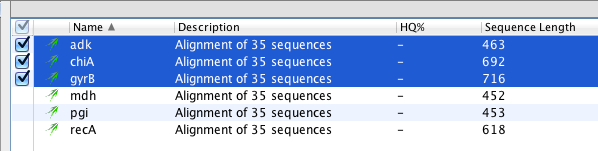
\includegraphics[resolution=120]{alignment_selection.png}

\hfill

Then navigating the menu to \texttt{Tools->Partition Allele Multiset}.


\hfill

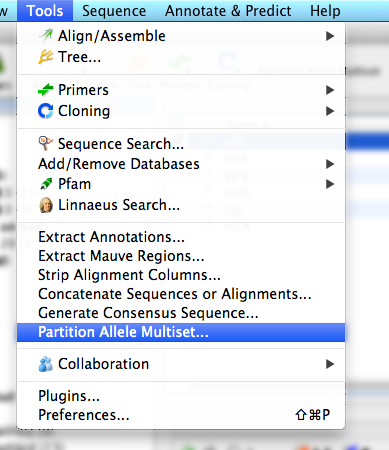
\includegraphics[resolution=130]{menu_entry.png}

\hfill

Then choosing options in the dialog box.

\hfill

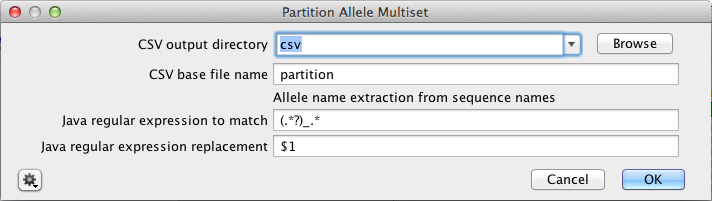
\includegraphics[resolution=130]{dialog_box.png}

\hfill

The meanings of the fields are as follows:

\begin{itemize}
\item \textit{CSV output directory} \hfill \\
\addcontentsline{toc}{subsubsection}{CSV output directory}
    This is the target directory into which the resulting table files will be
    written.  Note that pre-existing files of the same name as the output files
    will be overwritten without warning or prompting.

\item \textit{CSV base file name} \hfill \\
\addcontentsline{toc}{subsubsection}{CSV base file name}
    This is a string of text which will be appended with descriptive suffixes
    for each table.  For example the following entry,
    
    \begin{itemize}
    \item[]\texttt{partition1}
    \end{itemize}

    will result in the production of files such as these two,

    \begin{itemize}
    \item[]\texttt{partition1\_gene\_vs\_strain.csv}
    \item[]\texttt{partition1\_strain\_vs\_strain\_matrix.csv}
    \end{itemize}

\item \textit{Java regular expression to match} \hfill \\
\addcontentsline{toc}{subsubsection}{Java regular expression to match}
    %TODO

\item \textit{Java regular expression replacement} \hfill \\
\addcontentsline{toc}{subsubsection}{Java regular expression replacement}
    %TODO

\end{itemize}

\subsection{Example Regular Expressions}
    %TODO

\section{Description of Output Tables}
    %TODO

\end{document}
